\documentclass[tikz]{article}
\usepackage[utf8]{inputenc}
\usepackage[tmargin=2in]{geometry}
\usepackage{setspace}
\usepackage{verbatim}
\usepackage{listings}
\usepackage{amsmath}
\usepackage{amssymb}
\usepackage{pgfplots}
\usepackage{graphics}
\usepackage{csvsimple}
\usepackage{array}
\usepackage{longtable}
\usepackage{booktabs}
\usepackage{pgfplotstable}
\usepackage[toc,page]{appendix}
\usepackage{indentfirst}
\usepackage{float}
\usepackage{setspace}
\usetikzlibrary{positioning}

\doublespacing
\pagenumbering{gobble}

\pgfplotsset{every axis/.style={scale only axis}}

\begin{document}
\noindent
\textit{\textbf{Researcher:}} Dustin McAfee \\
\textbf{Presentation Title:} High Performance Clustering of Electroencephalogram (EEG) Data for Prediction of Seizure Events \\
\textbf{Institution:} University of Tennessee, Knoxville \\
\textbf{Department:} Department of Electrical Engineering and Computer Science \\

\singlespacing


\section{Abstract}


\begin{figure}[H]
	\centering
	\begin{tikzpicture}[yscale=0.8, xscale=0.8]
		\begin{axis}[legend style={at={(1,1)},anchor=north west},
		xlabel=k Pricipal Component,ylabel=Singular Value]
			\addplot[only marks, black, mark=*] table [x expr=\coordindex, y index=0, col sep=comma] {output/Singular_Values.txt};
		\end{axis}
	\end{tikzpicture}
	\caption{Scree Graph}
	\label{fig:scree}
\end{figure}

If $s_{i}$ is the $i$th principal component, then the amount of overall variance explained by $s_{i}$, denoted $r_{i}^{2}$, is computed using the below formula, Formula \ref{eq:1}.
\begin{equation}\label{eq:1}
r_{i}^{2} = \frac{s_{i}^{2}}{\sum_{j}s_{j}^{2}}
\end{equation}

These values are computed in "data.py", saved in the file, "Singular\_Values\_Percent\_Variance.txt", and plotted in a scatter plot as Figure \ref{fig:percent_var}, below.

\begin{figure}[H]
	\centering
	\begin{tikzpicture}[yscale=0.8, xscale=0.8]
		\begin{axis}[legend style={at={(1,1)},anchor=north west},
		xlabel=k Pricipal Component,ylabel=Percent Variance]
			\addplot[only marks, black, mark=*] table [x expr=\coordindex, y index=0, col sep=comma] {output/Singular_Values_Percent_Variance.txt};
		\end{axis}
	\end{tikzpicture}
	\caption{Percent Variance vs Principal Components}
	\label{fig:percent_var}
\end{figure}

The first 40 principal components cover about 95.88\% of the variance; looking at Figures \ref{fig:scree} and \ref{fig:percent_var} above, this looks to be a decent elbow point. The first two principal components are plotted against each other, and the projection of the Testing Dataset is color coded by category and shown below, in Figure \ref{fig:project}. Blue marks seizure moments.

\begin{figure}[H]
		\centering
	\begin{tikzpicture}[yscale=0.8, xscale=0.8]
		\begin{axis}[
			xtick pos=left,
			ytick pos=left,
			ztick pos=left,
			xlabel= First Principal Component,
			ylabel= Third Principal Component,
			zlabel= Second Principal Component,
		  ]
		\addplot3+[
			scatter/classes={0={blue}, 1={red}, 2={lightgray}, 3={green}, 4={yellow}}, 
			scatter, mark=*, only marks,
			scatter src=explicit symbolic,
			mark size=1.8,
			nodes near coords align={center},
		] table [x index=1, z index=2, y index=3, meta index=41, col sep=comma] 	{input/test/TestingData_Projected.txt};
		\legend{No Seizure,Seizure}
		\end{axis}
	\end{tikzpicture}
	\caption{Testing Dataset Projected onto first 3 Principal Components}
	\label{fig:project}
\end{figure}

The K-Means clustering algorithm is implemented in "kmeans.py," and takes one argument: $k$ number of clusters, (see "README.txt"). The initial values (seeds) for the centroids are chosen based on the K-Means++ algorithm \cite{kmeans++}. The first seed is chosen at random, then for each data point, $x$, the minimum difference between each $x$ and chosen centroids are used as weights for picking the next centroid. Each new centroid is chosen at random from the dataset, using the weighted probability distribution where the weights are proportional to the distances to the nearest centroid (See function "centroid" in "kmeans.py"). The purpose here is an attempt to initially start with clusters that are relatively spread out. The program converges when the sum of the differences of each centroid is less than 0.005. \\

The minimum intercluster distance and maximum intracluster distance are computed using the distance matrix. This algorithm is run for $k$ clusters, where $k = 2, 3$, on the standardized preprocessed numerical dataset projected onto the first 40 Principal Components. The maximum intercluster distance is computed using the maximum distance between any two points of different clusters, and similarly, the minumum intracluster distance is computed using the minimum of any two points of the same cluster. These two metrics, the Dunn index, and the number of iterations until convergence for each of the $k$ clusterings are reported in Figure \ref{fig:dunn1}, below.

\begin{figure}[H]
	\centering
	\begin{center}
		\begin{tabular}{|c|c|c|}
		\hline
		 & k=2 & k=3 \\
		\hline
		Min Inter & 9.94 & 0.74 \\
		\hline
		Max Intra & 92.77 & 91.71 \\
		\hline
		Dunn & 0.0963 & 0.0080 \\
		\hline
		\# Iterations & 20 & 27 \\
		\hline
		\end{tabular} \\
		\caption{Dunn index for different K values on Projected Training Dataset}
		\label{fig:dunn1}
	\end{center}
\end{figure}

\begin{figure}[H]
	\centering
	\begin{center}
		\begin{tabular}{|c|c|c|}
		\hline
		 & k=2 & k=3 \\
		\hline
		Min Inter & 1.47 & 0.39 \\
		\hline
		Max Intra & 89.69 & 86.68 \\
		\hline
		Dunn & 0.0164 & 0.0045 \\
		\hline
		\end{tabular} \\
		\caption{Dunn index for different K values on Projected Testing Dataset}
		\label{fig:dunn2}
	\end{center}
\end{figure}


\begin{figure}[H]
	\begin{center}
		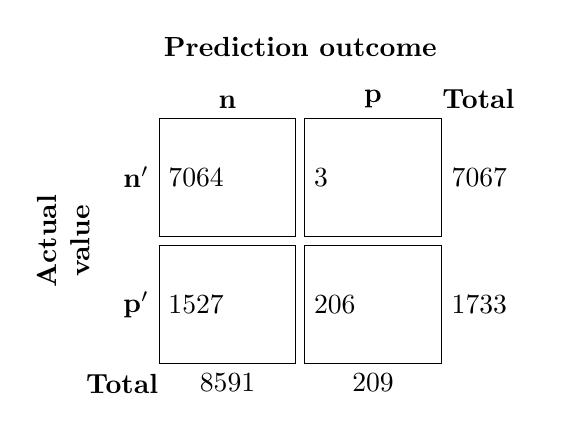
\begin{tikzpicture}[
			box/.style={draw,rectangle,minimum size=1.5cm,text width=1.5cm,align=left}]
			\matrix (conmat) [row sep=.1cm,column sep=.1cm] {
				\node (tneg) [box,
    				label=left:\( \mathbf{n'} \),
    				label=above:\( \mathbf{n} \),
    			] {7064};
				&

				\node (fpos) [box,
				    label=above:\textbf{p},
    				label=above right:\textbf{Total},
    				label=right:\( 7067 \)] {3};
				\\
				\node (fneg) [box,
    				label=left:\( \mathbf{p'} \),
    				label=below left:\textbf{Total},
    				label=below:8591] {1527};
				&
				\node (tpos) [box,
				    label=right:\( 1733 \),
				    label=below:209] {206};
				\\
			};
			\node [rotate=90,left=.05cm of conmat,anchor=center,text width=1.5cm,align=center] {\textbf{Actual \\ value}};
			\node [above=.05cm of conmat] {\textbf{Prediction outcome}};
		\end{tikzpicture}
	\caption{Confusion Matrix for K = 2 on Projected Training Dataset (82.61\% Accuracy, 11.86\% Sensitivity)}
	\label{fig:confusion_kmeans2}
	\end{center}
\end{figure}

\begin{figure}[H]
	\begin{center}
		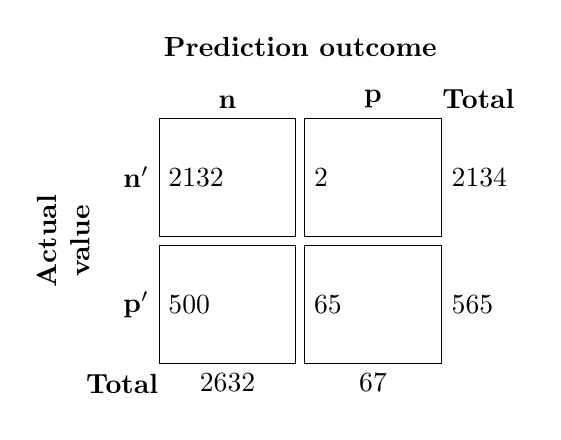
\begin{tikzpicture}[
			box/.style={draw,rectangle,minimum size=1.5cm,text width=1.5cm,align=left}]
			\matrix (conmat) [row sep=.1cm,column sep=.1cm] {
				\node (tneg) [box,
    				label=left:\( \mathbf{n'} \),
    				label=above:\( \mathbf{n} \),
    			] {2132};
				&

				\node (fpos) [box,
				    label=above:\textbf{p},
    				label=above right:\textbf{Total},
    				label=right:\( 2134 \)] {2};
				\\
				\node (fneg) [box,
    				label=left:\( \mathbf{p'} \),
    				label=below left:\textbf{Total},
    				label=below:2632] {500};
				&
				\node (tpos) [box,
				    label=right:\( 565 \),
				    label=below:67] {65};
				\\
			};
			\node [rotate=90,left=.05cm of conmat,anchor=center,text width=1.5cm,align=center] {\textbf{Actual \\ value}};
			\node [above=.05cm of conmat] {\textbf{Prediction outcome}};
		\end{tikzpicture}
	\caption{Confusion Matrix for K = 2 on Projected Testing Dataset (81.44\% Accuracy, 11.66\% Sensitivity)}
	\label{fig:confusion_kmeans2_test}
	\end{center}
\end{figure}

\begin{figure}[H]
	\begin{center}
		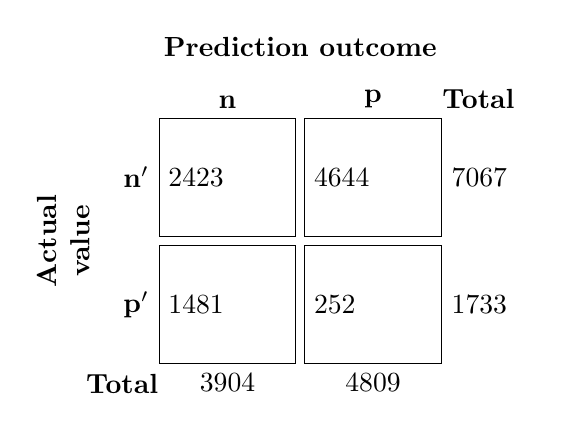
\begin{tikzpicture}[
			box/.style={draw,rectangle,minimum size=1.5cm,text width=1.5cm,align=left}]
			\matrix (conmat) [row sep=.1cm,column sep=.1cm] {
				\node (tneg) [box,
    				label=left:\( \mathbf{n'} \),
    				label=above:\( \mathbf{n} \),
    			] {2423};
				&

				\node (fpos) [box,
				    label=above:\textbf{p},
    				label=above right:\textbf{Total},
    				label=right:\( 7067 \)] {4644};
				\\
				\node (fneg) [box,
    				label=left:\( \mathbf{p'} \),
    				label=below left:\textbf{Total},
    				label=below:3904] {1481};
				&
				\node (tpos) [box,
				    label=right:\( 1733 \),
				    label=below:4809] {252};
				\\
			};
			\node [rotate=90,left=.05cm of conmat,anchor=center,text width=1.5cm,align=center] {\textbf{Actual \\ value}};
			\node [above=.05cm of conmat] {\textbf{Prediction outcome}};
		\end{tikzpicture}
	\caption{Confusion Matrix for K = 3 on Projected Training Dataset (30.40\% Accuracy, 14.54\% Sensitivity)}
	\label{fig:confusion_kmeans3}
	\end{center}
\end{figure}

\begin{figure}[H]
	\begin{center}
		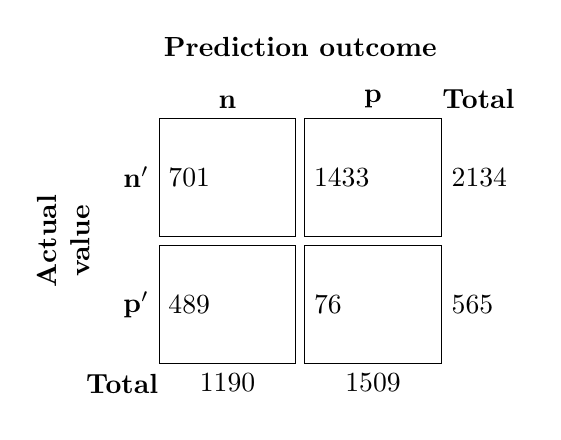
\begin{tikzpicture}[
			box/.style={draw,rectangle,minimum size=1.5cm,text width=1.5cm,align=left}]
			\matrix (conmat) [row sep=.1cm,column sep=.1cm] {
				\node (tneg) [box,
    				label=left:\( \mathbf{n'} \),
    				label=above:\( \mathbf{n} \),
    			] {701};
				&
				\node (fpos) [box,
				    label=above:\textbf{p},
    				label=above right:\textbf{Total},
    				label=right:\( 2134 \)] {1433};
				\\
				\node (fneg) [box,
    				label=left:\( \mathbf{p'} \),
    				label=below left:\textbf{Total},
    				label=below:1190] {489};
				&
				\node (tpos) [box,
				    label=right:\( 565 \),
				    label=below:1509] {76};
				\\
			};
			\node [rotate=90,left=.05cm of conmat,anchor=center,text width=1.5cm,align=center] {\textbf{Actual \\ value}};
			\node [above=.05cm of conmat] {\textbf{Prediction outcome}};
		\end{tikzpicture}
	\caption{Confusion Matrix for K = 3 on Projected Testing Dataset (28.79\% Accuracy, 13.45\% Sensitivity)}
	\label{fig:confusion_kmeans3_test}
	\end{center}
\end{figure}

The K-Means clustering of the preprocessed training dataset for 2 (3) clusters is saved in the file "Data\_Kmeans\_2.txt" ("Data\_Kmeans\_3.txt"), and the clusters are color coded and plotted against the testing dataset projected onto the first 3 principal components (see files "TestingData\_Kmeans\_2.txt" and "TestingData\_Kmeans\_3.txt") in Figure \ref{fig:kmean2} (Figure \ref{fig:kmean3}), below. 

\begin{figure}[H]
		\centering
	\begin{tikzpicture}[yscale=0.8, xscale=0.8]
		\begin{axis}[
			xtick pos=left,
			ytick pos=left,
			ztick pos=left,
			xlabel= First Principal Component,
			ylabel= Third Principal Component,
			zlabel= Second Principal Component,
		  ]
		\addplot3+[
			scatter/classes={0={blue}, 1={red}, 2={lightgray}, 3={green}, 4={yellow}, 5={purple}}, 
			scatter, mark=*, only marks,
			scatter src=explicit symbolic,
			mark size=1.8,
			nodes near coords align={center},
		] table [x index=1, y index=2, z index=3, meta index=0, col sep=comma] 	{output/TestingData_Kmeans_2.txt};
		\end{axis}
	\end{tikzpicture}
	\caption{K-Means Clustering (K=2) of Standardized Testing Dataset vs First 3 Principal Components}
	\label{fig:kmean2}
\end{figure}

\begin{figure}[H]
		\centering
	\begin{tikzpicture}[yscale=0.8, xscale=0.8]
		\begin{axis}[
			xtick pos=left,
			ytick pos=left,
			ztick pos=left,
			xlabel= First Principal Component,
			ylabel= Third Principal Component,
			zlabel= Second Principal Component,
		  ]
		\addplot3+[
			scatter/classes={0={blue}, 1={red}, 2={lightgray}, 3={green}, 4={yellow}, 5={purple}}, 
			scatter, mark=*, only marks,
			scatter src=explicit symbolic,
			mark size=1.8,
			nodes near coords align={center},
		] table [x index=1, y index=2, z index=3, meta index=0, col sep=comma] 	{output/TestingData_Kmeans_3.txt};
		\end{axis}
	\end{tikzpicture}
	\caption{K-Means Clustering (K=3) of Standardized Testing Dataset vs First 3 Principal Components}
	\label{fig:kmean3}
\end{figure}

The Expectation Maximization algorithm assumes Gaussian models for each cluster. The program ("exmax.py") borrows a few functions from the K-Means program ("kmeans.py"), such as the initialization of the centroids (the K-Means++ method \cite{kmeans++}), assigning points to labels, and calculating the sum of changes in the centroids. Similarly to the K-Means program, the Expectation Maximization program converges when the sum of changes in the centroids are less than 0.005

This program is run on different sized clusters. Contrast to the K-Means algorithm, the Dunn index is not a good index for validation of clusters of Gaussian distributions, so a different index is used for validation of the clusters in this case. Instead of using the ratio of minimum intercluster distance to maximum intracluster distance (which is good for spherical distributions), the index chosen is the Silhouette index. To compute this index, the average intracluster distance, $a(i)$ is calculated per data point, $i$. The smallest average intercluster distance, $b(i)$, per data point, $i$, is also computed. Equation \ref{eq:2}, below, computes the Silhouette index per data point (see function "avg\_sil\_index" in "exmax.py").

\begin{equation}\label{eq:2}
\frac{b(i) - a(i)}{\text{max}\{a(i), b(i)\}}
\end{equation}

This value is averaged over the entire dataset to produce the Silhouette index for the dataset, which better measures how appropriately the data has been clustered for the Gaussian clusters.

To this end, $k=2,3$ clusters are run and their respective Silhouette indices and number of iterations are reported in Figure \ref{fig:sil}, below.

\begin{figure}[H]
	\begin{center}
		\begin{tabular}{|c|c|c|}
		\hline
		k & k=2 & k=3 \\
		\hline
		Silhouette & 0.3789 & 0.0580 \\
		\hline
		\# Iterations & 13 & 14 \\
		\hline
		\end{tabular} \\
		\caption{Silhouette indices for Training Dataset k values}
		\label{fig:sil_train}
	\end{center}
\end{figure}

\begin{figure}[H]
	\begin{center}
		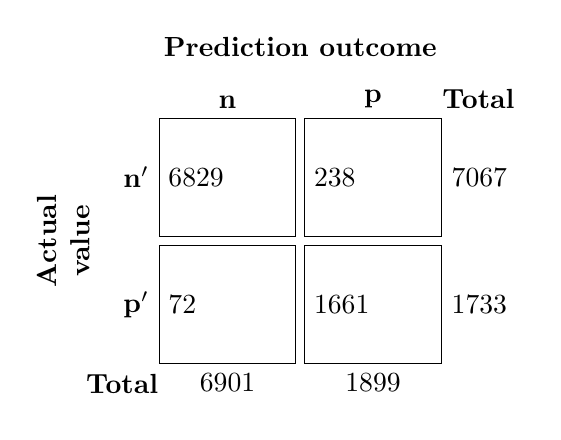
\begin{tikzpicture}[
			box/.style={draw,rectangle,minimum size=1.5cm,text width=1.5cm,align=left}]
			\matrix (conmat) [row sep=.1cm,column sep=.1cm] {
				\node (tneg) [box,
    				label=left:\( \mathbf{n'} \),
    				label=above:\( \mathbf{n} \),
    			] {6829};
				&
				\node (fpos) [box,
				    label=above:\textbf{p},
    				label=above right:\textbf{Total},
    				label=right:\( 7067 \)] {238};
				\\
				\node (fneg) [box,
    				label=left:\( \mathbf{p'} \),
    				label=below left:\textbf{Total},
    				label=below:6901] {72};
				&
				\node (tpos) [box,
				    label=right:\( 1733 \),
				    label=below:1899] {1661};
				\\
			};
			\node [rotate=90,left=.05cm of conmat,anchor=center,text width=1.5cm,align=center] {\textbf{Actual \\ value}};
			\node [above=.05cm of conmat] {\textbf{Prediction outcome}};
		\end{tikzpicture}
	\caption{Confusion Matrix for K = 2 on Projected Training Dataset (96.48\% Accuracy, 95.85\% Sensitivity)}
	\label{fig:confusion_em2}
	\end{center}
\end{figure}

\begin{figure}[H]
	\begin{center}
		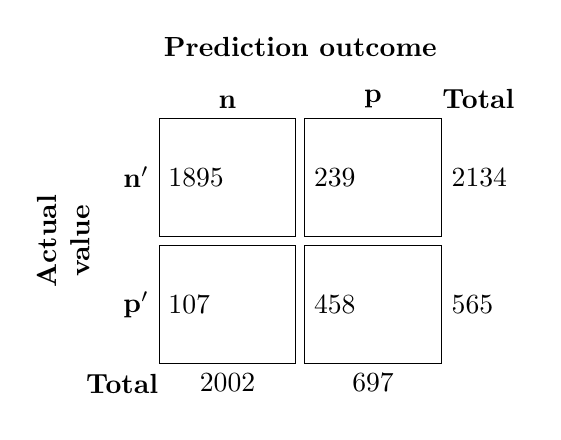
\begin{tikzpicture}[
			box/.style={draw,rectangle,minimum size=1.5cm,text width=1.5cm,align=left}]
			\matrix (conmat) [row sep=.1cm,column sep=.1cm] {
				\node (tneg) [box,
    				label=left:\( \mathbf{n'} \),
    				label=above:\( \mathbf{n} \),
    			] {1895};
				&
				\node (fpos) [box,
				    label=above:\textbf{p},
    				label=above right:\textbf{Total},
    				label=right:\( 2134 \)] {239};
				\\
				\node (fneg) [box,
    				label=left:\( \mathbf{p'} \),
    				label=below left:\textbf{Total},
    				label=below:2002] {107};
				&
				\node (tpos) [box,
				    label=right:\( 565 \),
				    label=below:697] {458};
				\\
			};
			\node [rotate=90,left=.05cm of conmat,anchor=center,text width=1.5cm,align=center] {\textbf{Actual \\ value}};
			\node [above=.05cm of conmat] {\textbf{Prediction outcome}};
		\end{tikzpicture}
	\caption{Confusion Matrix for K = 2 on Projected Testing Dataset (87.22\% Accuracy, 81.10\% Sensitivity)}
	\label{fig:confusion_em2_test}
	\end{center}
\end{figure}

\begin{figure}[H]
	\begin{center}
		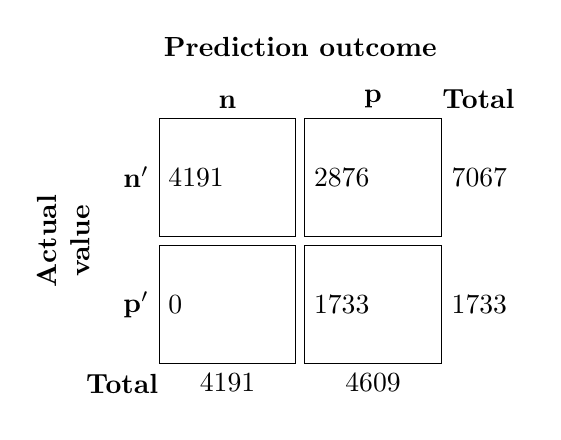
\begin{tikzpicture}[
			box/.style={draw,rectangle,minimum size=1.5cm,text width=1.5cm,align=left}]
			\matrix (conmat) [row sep=.1cm,column sep=.1cm] {
				\node (tneg) [box,
    				label=left:\( \mathbf{n'} \),
    				label=above:\( \mathbf{n} \),
    			] {4191};
				&

				\node (fpos) [box,
				    label=above:\textbf{p},
    				label=above right:\textbf{Total},
    				label=right:\( 7067 \)] {2876};
				\\
				\node (fneg) [box,
    				label=left:\( \mathbf{p'} \),
    				label=below left:\textbf{Total},
    				label=below:4191] {0};
				&
				\node (tpos) [box,
				    label=right:\( 1733 \),
				    label=below:4609] {1733};
				\\
			};
			\node [rotate=90,left=.05cm of conmat,anchor=center,text width=1.5cm,align=center] {\textbf{Actual \\ value}};
			\node [above=.05cm of conmat] {\textbf{Prediction outcome}};
		\end{tikzpicture}
	\caption{Confusion Matrix for K = 3 on Projected Training Dataset (67.32\% Accuracy, 100\% Sensitivity)}
	\label{fig:confusion_em3}
	\end{center}
\end{figure}

\begin{figure}[H]
	\begin{center}
		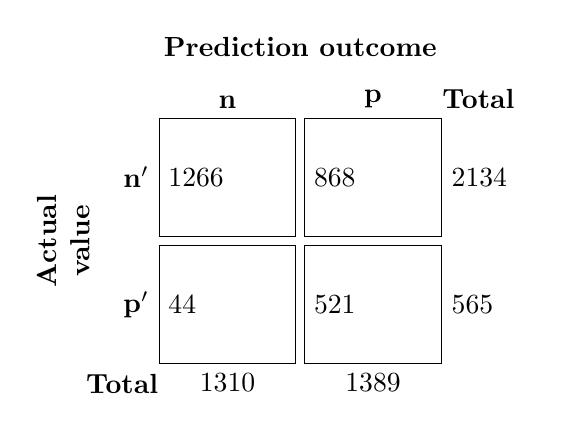
\begin{tikzpicture}[
			box/.style={draw,rectangle,minimum size=1.5cm,text width=1.5cm,align=left}]
			\matrix (conmat) [row sep=.1cm,column sep=.1cm] {
				\node (tneg) [box,
    				label=left:\( \mathbf{n'} \),
    				label=above:\( \mathbf{n} \),
    			] {1266};
				&
				\node (fpos) [box,
				    label=above:\textbf{p},
    				label=above right:\textbf{Total},
    				label=right:\( 2134 \)] {868};
				\\
				\node (fneg) [box,
    				label=left:\( \mathbf{p'} \),
    				label=below left:\textbf{Total},
    				label=below:1310] {44};
				&
				\node (tpos) [box,
				    label=right:\( 565 \),
				    label=below:1389] {521};
				\\
			};
			\node [rotate=90,left=.05cm of conmat,anchor=center,text width=1.5cm,align=center] {\textbf{Actual \\ value}};
			\node [above=.05cm of conmat] {\textbf{Prediction outcome}};
		\end{tikzpicture}
	\caption{Confusion Matrix for K = 3 on Projected Testing Dataset (66.25\% Accuracy, 92.23\% Sensitivity)}
	\label{fig:confusion_em3_test}
	\end{center}
\end{figure}








Figures \ref{fig:me2} and \ref{fig:me3}, below, show clusterings using the Gaussian Mixture Expectation Maximization model run on the dataset projected onto the first 40 principal components with $k$=2 and $k$=3 (saved in files "Data\_EM\_2.txt" and "Data\_EM\_3.txt"), respectively.

\begin{figure}[H]
		\centering
	\begin{tikzpicture}[yscale=0.8, xscale=0.8]
		\begin{axis}[
			xtick pos=left,
			ytick pos=left,
			ztick pos=left,
			xlabel= First Principal Component,
			ylabel= Third Principal Component,
			zlabel= Second Principal Component,
		  ]
		\addplot3+[
			scatter/classes={0={blue}, 1={red}, 2={lightgray}},
 			scatter, mark=*, only marks,
			scatter src=explicit symbolic,
			mark size=1.8,
			nodes near coords align={center},
		] table [x index=1, y index=2, z index=3, meta index=0, col sep=comma] 	{output/TestingData_EM_2.txt};
		\end{axis}
	\end{tikzpicture}
	\caption{EM Clustering (K=2) of Standardized Testing Dataset Projected onto First 3 Principal Components}
	\label{fig:me2}
\end{figure}
\begin{figure}[H]
		\centering
	\begin{tikzpicture}[yscale=0.8, xscale=0.8]
		\begin{axis}[
			xtick pos=left,
			ytick pos=left,
			ztick pos=left,
			xlabel= First Principal Component,
			ylabel= Third Principal Component,
			zlabel= Second Principal Component,
		  ]
		\addplot3+[
			scatter/classes={0={blue}, 1={red}, 2={lightgray}},
 			scatter, mark=*, only marks,
			scatter src=explicit symbolic,
			mark size=1.8,
			nodes near coords align={center},
		] table [x index=1, y index=2, z index=3, meta index=0, col sep=comma] 	{output/TestingData_EM_3.txt};
		\end{axis}
	\end{tikzpicture}
	\caption{EM Clustering (K=3) of Standardized Testing Dataset Projected onto First 3 Principal Components}
	\label{fig:me3}
\end{figure}


\begin{thebibliography}{666}
\bibitem{kmeans++}
Arthur, David \& Vassilvitskii, Sergei. (2007). K-Means++: The Advantages of Careful Seeding. Proc. of the Annu. ACM-SIAM Symp. on Discrete Algorithms. 8. 1027-1035. 10.1145/1283383.1283494. 
\end{thebibliography}

\begin{appendices}
\section{Three Dimensional Plots}
\label{sec:appendix}

\begin{figure}[H]
		\centering
	\begin{tikzpicture}[yscale=0.8, xscale=0.8]
		\begin{axis}[
			xtick pos=left,
			ytick pos=left,
			ztick pos=left,
			xlabel= First Principal Component,
			ylabel= Third Principal Component,
			zlabel= Second Principal Component,
		  ]
		\addplot3+[
			scatter/classes={0={blue}, 1={red}, 2={lightgray}, 3={green}, 4={yellow}}, 
			scatter, mark=*, only marks,
			scatter src=explicit symbolic,
			mark size=1.8,
			nodes near coords align={center},
		] table [x index=1, z index=2, y index=3, meta index=0, col sep=comma] 	{output/TestingData_Kmeans_2.txt};
		\end{axis}
	\end{tikzpicture}
	\caption{K-Means Clustering (K=2) of Standardized Data vs First 3 Principal Components}
	\label{fig:kmean2_3d}
\end{figure}


\end{appendices}

\end{document}

